\documentclass[fleqn,useAMS,usenatbib]{mnras}
%=====================================================================
% CUSTOM: PACKAGES, MACROS & SETTINGS
%=====================================================================
% packages for figures
\usepackage{graphicx,todonotes}

% packages for symbols
\usepackage{latexsym,amssymb}

% AMS-LaTeX package for e.g. subequations
\usepackage{amsmath,morefloats}
\usepackage{natbib,graphicx,amsmath,subfigure,color,xcolor,hyperref}

\topmargin-1cm

\graphicspath{{figures/}}

\newcommand\notedo[1]{\todo[color=yellow, inline, size=\small]{To do:#1}}
\newcommand\notewrite[1]{\todo[color=orange, inline, size=\small]{To write: #1}}
\newcommand\noteask[1]{\todo[color=cyan, inline, size=\small]{To ask: #1}}
\newcommand\notecontrib[1]{\todo[color=green, inline, size=\small]{Contributors: #1}}
\newcommand\esstodo[1]{\todo[color=yellow, inline, size=\small]{ESS: #1}}
\newcommand{\ess}[1]{\textcolor{red}{[ESS: \bf #1]}}
\newcommand{\mrb}[1]{\textcolor{purple}{[MRB: \bf #1]}}


\newcommand{\vecg}{\mbox{\boldmath $g$}}
\newcommand{\vece}{\mbox{\boldmath $e$}}
\newcommand{\veck}{\mbox{\boldmath $k$}}
\newcommand{\vecQ}{\mbox{\boldmath $Q$}}
\newcommand{\vecF}{\mbox{\boldmath $F$}}
\newcommand{\vecD}{\mbox{\boldmath $D$}}
\newcommand{\matR}{\mbox{$\bf R$}}
\newcommand{\matC}{\mbox{$\bf C$}}
\newcommand{\bnab}{\boldsymbol{\nabla}}
\newcommand{\bnabg}{\boldsymbol{\nabla_g}}
\newcommand{\galsim}{\texttt{GALSIM}}
\newcommand{\ngmix}{\texttt{ngmix}}
\newcommand{\nnsim}{\texttt{nsim}}
\newcommand{\snr}{$S/N$}
\newcommand{\sn}{$S/N$}
\newcommand{\coadd}{{\rm coadd}}
\newcommand{\desreq}{$4\times 10^{-3}$}
\newcommand{\lsstreq}{$2\times 10^{-3}$}

\newcommand{\mcal}{\textsc{metacalibration}}
\newcommand{\mdet}{\textsc{metadetection}}
\newcommand{\Mcalshort}{\textsc{metacal}}
\newcommand{\Mcal}{\textsc{Metacalibration}}
\newcommand{\vest}{\mbox{\boldmath $e$}}
\newcommand{\est}{e}
\newcommand{\mcalR}{\mbox{\boldmath $R$}}
\newcommand{\mcalRS}{\mbox{\boldmath $R_S$}}
\newcommand{\gest}{\mbox{\boldmath $\hat \gamma$}}
\newcommand{\vecgam}{\mbox{\boldmath $\gamma$}}

\newcommand{\sx}{\textsc{SExtractor}}

\newcommand{\bfd}{\textsc{BFD}}

\newcommand{\vonkarman}{{von K\'arm\'an}~}

\title[Metadetection]{Mitigating Shear-dependent Detection Biases with \Mcal}

\author[Sheldon et~al.]{Erin Sheldon$^1$, Matthew R. Becker$^2$,
Niall MacCrann$^{3,4}$, Michael Jarvis$^5$
  \\$^1$Brookhaven National Laboratory, Bldg. 510, Upton, NY 11973, USA
  \\$^2$High Energy Physics Division, Argonne National Laboratory , Lemont, IL 60439, USA
  \\$^3$Center for Cosmology and Astro-Particle Physics, The Ohio State University, Columbus, OH 43210, USA
  \\$^4$Department of Physics, The Ohio State University, Columbus, OH 43210, USA
  \\$^5$Department of Physics and Astronomy, University of Pennsylvania, Philadelphia, PA 19104, USA
}

\begin{document}
\date{Draft \today}
\maketitle

\begin{abstract}

\Mcal\ is a new technique for measuring weak gravitational lensing shear that
is unbiased for isolated galaxy images.  In this work we test the \mcal\ method
with overlapping, or ``blended'' galaxy images.  Using standard \mcal\ we find
a significant shear calibration bias when objects overlap. This bias is a few
percent for galaxy densities relevant for current surveys, and increases to
tens of percent for future surveys.  This bias is due to shear-dependent
detection rather than blending itself; if detection is shear independent, no
de-blending of images is needed, in principle.  We demonstrate that
shear-dependent detection biases are accurately removed when including
detection in the \mcal\ process.

\end{abstract}

\section{Introduction}


Recently introduced methods for the estimation of weak gravitational lensing
shear promise to provide calibration at the 0.1\% level, adequate for the
requirements of future weak lensing surveys.  Two methods that have
demonstrated sufficient accuracy without the use of calibration from
simulations, and without any compromise of precision, are the \bfd\ method
\citep{BernBFD2016} and the \mcal\ method \citep{HuffMcal2017,SheldonMcal2017}.
The tests of these methods, while stringent, did not include an important
aspect of the real universe: the images of objects overlap on the sky. In this
work we test \mcal\ in the presence of blending, and demonstrate that there is
a bias associated with shear-dependent detection.  We introduce an improvement
to the method that naturally accounts for this shear-dependent detection bias.

%Proper accounting for blending is crucial for obtaining accurate redshifts
%distributions, which are required to interpret the lensing signal (XXX good
%citation)?

Weak lensing measurements typically involve measurement of some kind of
ellipticity or second moments of a galaxy light profile.  Blending will produce
biases and increased variance in these measurements \citep{DawsonBlending2016}.

A method such as \mcal\ can in principle calibrate any measurement biases, even
those associated with blending.  More problematic for shear calibration is the
dependence of the object detection on shear.  Because the shear transformation
is a simple mapping in the weak shear regime, and the mapping preserves surface
brightness \citep{SchneiderBook92}, detection need not be shear dependent.  For
example, a detection algorithm that simply identifies connected regions above a
threshold as a single object will not in principle be shear dependent. However,
in real observations the image is smeared by a point-spread-function (PSF) due
to the atmosphere, telescope optics or detector. In this case the overlap of
objects does depend on shear because the PSF convolution occurs after the shear
mapping.  This effect is demonstrated in figure \ref{fig:toy}.  In this case
the simple threshold detection method mentioned above will manifest a
shear-dependent detection bias.


\begin{figure*}
    %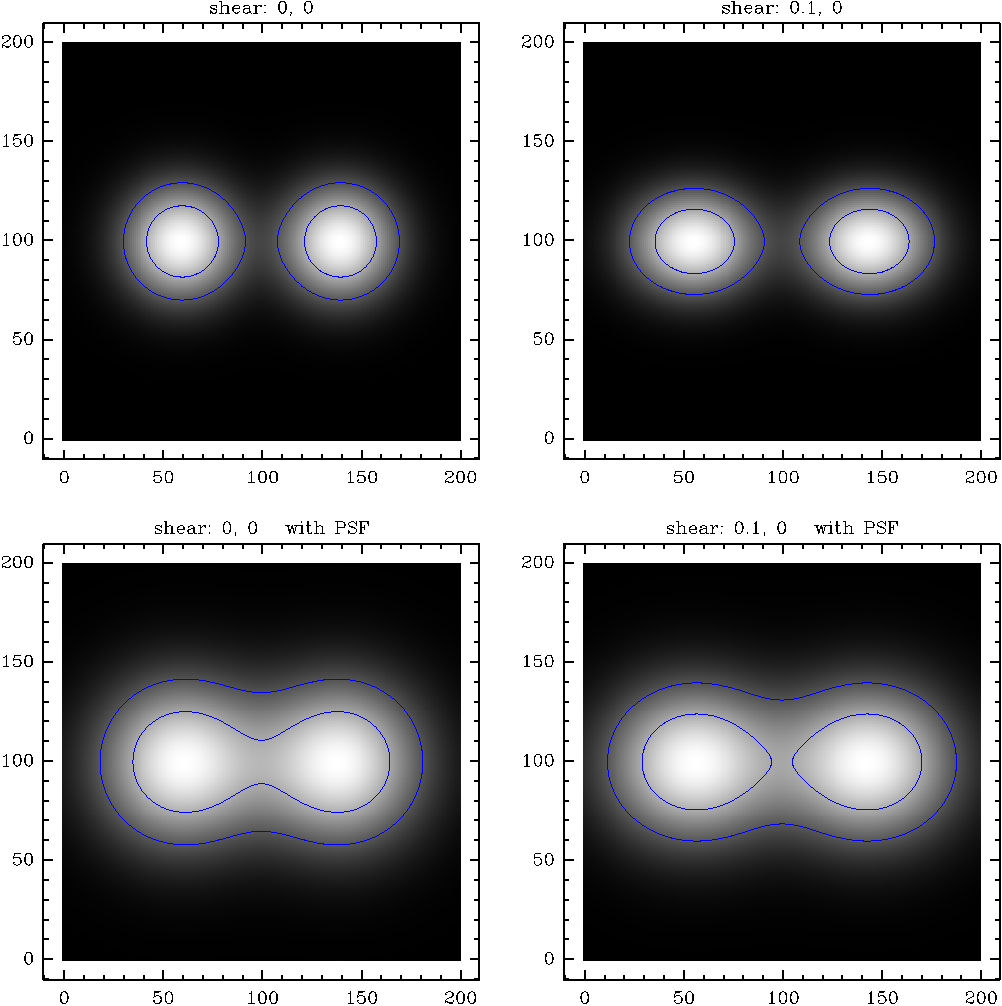
\includegraphics[width=\textwidth]{figures/toy.pdf}
    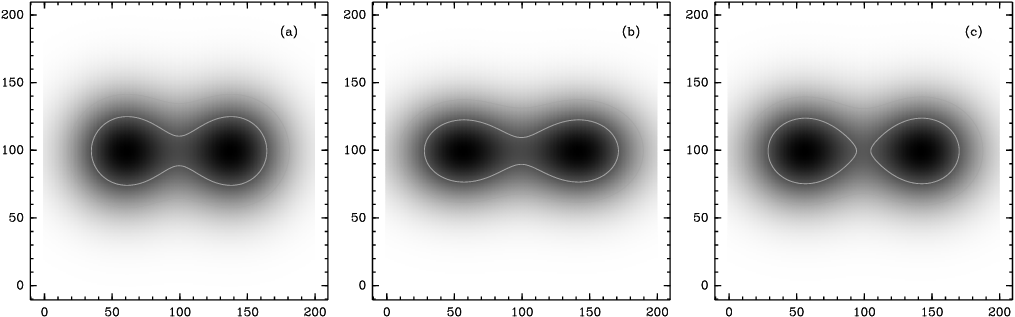
\includegraphics[width=\textwidth]{figures/toy.png}

    \caption{ Toy example of shear-dependent detection in the presence of a
    PSF.  In panel (a) two objects are present, convolved by a PSF with no
    shear.  Contours represent constant brightness.  In panel (b) the objects
    are shared by a shear $(0.0, 0.1)$ {\em after} the PSF convolution.
    Contours are the same as panel (a).  In this case the inner contours for
    the two objects overlap before and after application of the shear.  This is
    a general property of the shear transformation in the weak regime.   In
    panel (c) the shear is applied {\em before} the PSF convolution, which
    mimics real sky images.  In this case the inner contours do not overlap
    after shearing.  For case (c) a detection algorithm that identified
    connected regions above a threshold as a single object would manifest a
    shear-dependent detection bias.  \label{fig:toy} }

\end{figure*}

Common detection schemes in use today, such at those in Source Extractor
\citep{Bertin96} and the HST/LSST pipelines \citep{BoschHSC2018,BoschLSST2018}
are based on thresholding, similar to the simple approach described above but
differing in complexity and efficiency.  Thus we would expect detections
produced by those codes to also manifest shear dependence.

Any shear-dependent measurement effects can in principle be taken into account
within the \mcal\ formalism.  However, the implementations presented in
\cite{HuffMcal2017} and \cite{SheldonMcal2017} work by applying artificial
shears to small postage stamp images for objects found in an {\em independent}
detection step.  Corrections for selection effects were derived in
\cite{SheldonMcal2017}, but those do not work near the detection threshold if
detection is not included as part of the \mcal\ process.  As we will
demonstrate, detection effects can incorporated naturally by shearing larger
images, rather than small postage stamps, and re-running the detection phase on
each of the sheared images. In this process, shear measurement errors,
selection effects and detection effects are all accounted for.  There are
number of technical challenges associated with this \mcal\ implementation,
which we will address in turn.

The paper is laid out as follows.... blah blah.


\section{\textsc{METACALIBRATION}}

blah

\section{MOF Deblending}

blah

\section{Simulations}

\subsection{Galaxy Pairs} \label{sec:pairs}

We will first show tests with two simulated galaxies at various separations,
similar to the case shown in figure \ref{fig:toy}.  The galaxies were each a
combination of a bulge component, modeled as a De Vaucouleurs' profile
\citep{devauc1948} and disk component modeled as an exponential.

The fraction of light in the bulge was random and ranged uniformly between 0.0
and 1.0. The disk ellipticity was drawn from the distribution presented in
\cite{ba14}, equation 24, with ellipticity variance set to 0.20, with a random
orientation.  The bulge was given the same orientation as the disk but with
ellipticity set to the disk ellipticity times a random number drawn uniformly
between 0.0 and 0.5.  The half light radius of the disk
$r_{50}^{\mathrm{disk}}$ was set to a uniform random draw between 0.4 and 0.6
arcsec; that of the bulge was a random draw between $0.4
r_{50}^{\mathrm{disk}}$ and $0.6 r_{50}^{\mathrm{disk}}$.  The bulge was
shifted from the center of the disk within a radius
0.05$r_{50}^{\mathrm{disk}}$ and in a random direction.

The light of the disk was divided between a smooth component and a set of
simulated ``knots of star formation'', represented by point sources placed
randomly with the same exponential distribution as the disk.  Between 1 and 50
knots were placed, such that the fraction light in the knots ranged between
0.4\% and 20\%.

The total flux and noise were set such that the signal-to-noise ratio ranged
uniformly between 25 and 35.

Two of these randomly generated galaxies were placed in an image, with
separation ranging from 1.0 and 4.0 arcsec. The pair were placed such that the
mid-point between them corresponded to the center of the image, and the line
between the pair had a random random orientation relative to the coordinate
axes.  Each object was given an additional random dither within a pixel.
The galaxies were treated as totally transparent, such that the value in
a pixel was equal to the total sum from both galaxies plus noise.

All images were generated using the \texttt{GALSIM} software package
\citep{GALSIM2015}, with pixel scale of 0.263 arcseconds.

Example images are shown in figure \ref{fig:pairs}

\begin{figure*}
    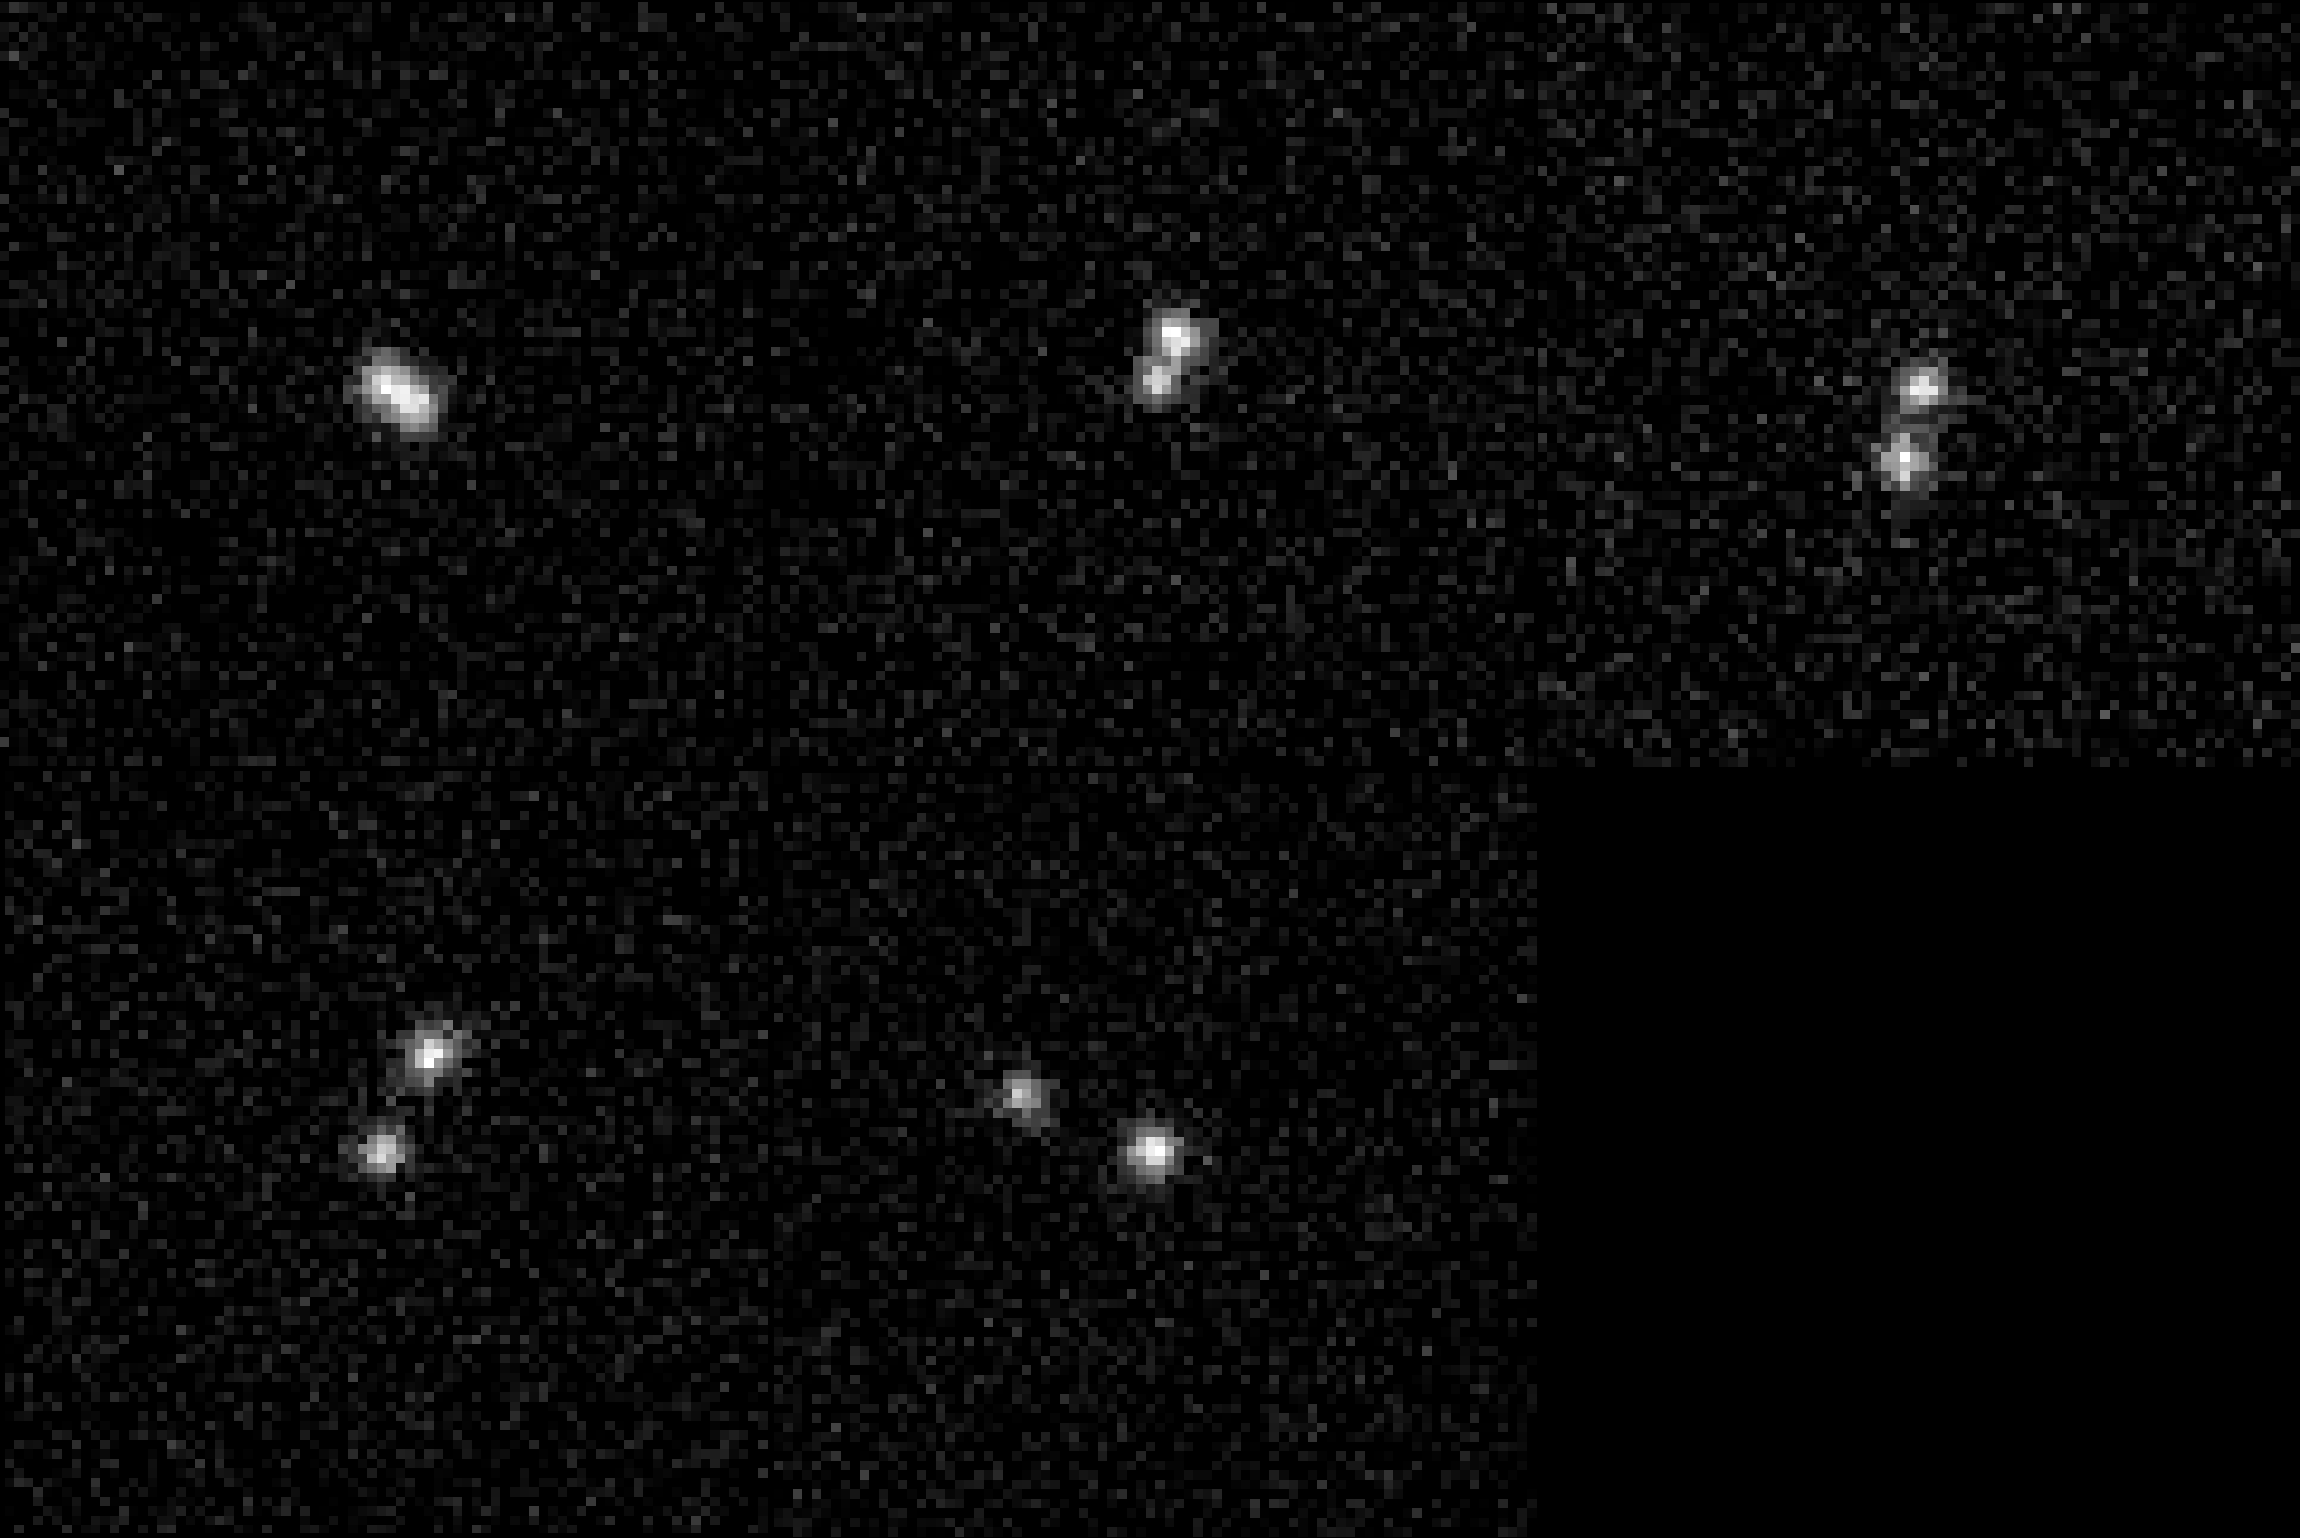
\includegraphics[width=\textwidth]{figures/bdk-comb.png}

    \caption{ Example images of simulated galaxies used for the pair tests
    presented in section \ref{sec:pairs}.  From left to right in the top row,
    the separations are 1.0, 1.5, 2.0. From left to right in the bottom row the
    separations are 3.0 and 4.0 arscec. The pixel scale is 0.263 arcsec.
    \label{fig:pairs} }

\end{figure*}


\subsection{Simulations with Representative Galaxy Density and Noise}

\begin{figure*}
    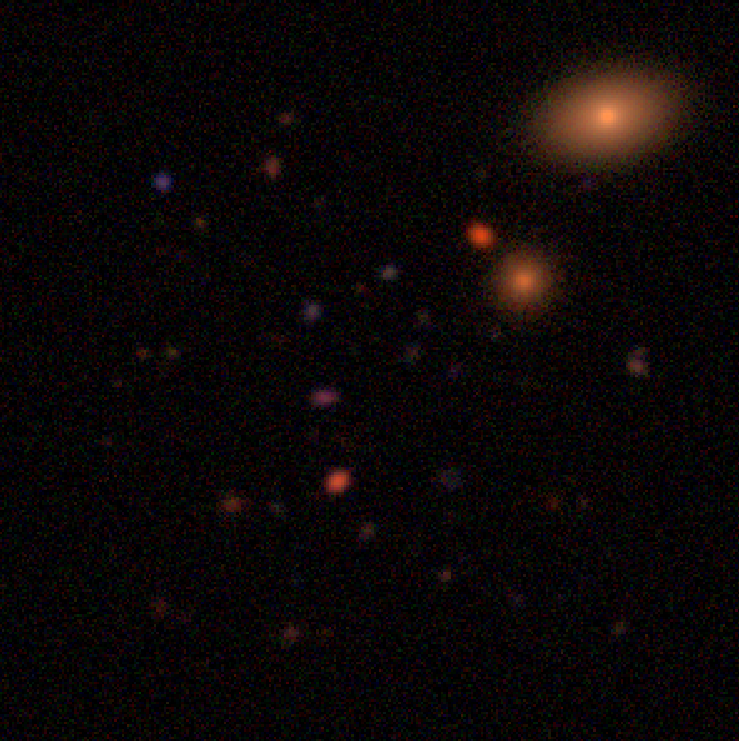
\includegraphics[width=0.9\columnwidth]{figures/des-rgb-000000-crop.png}
    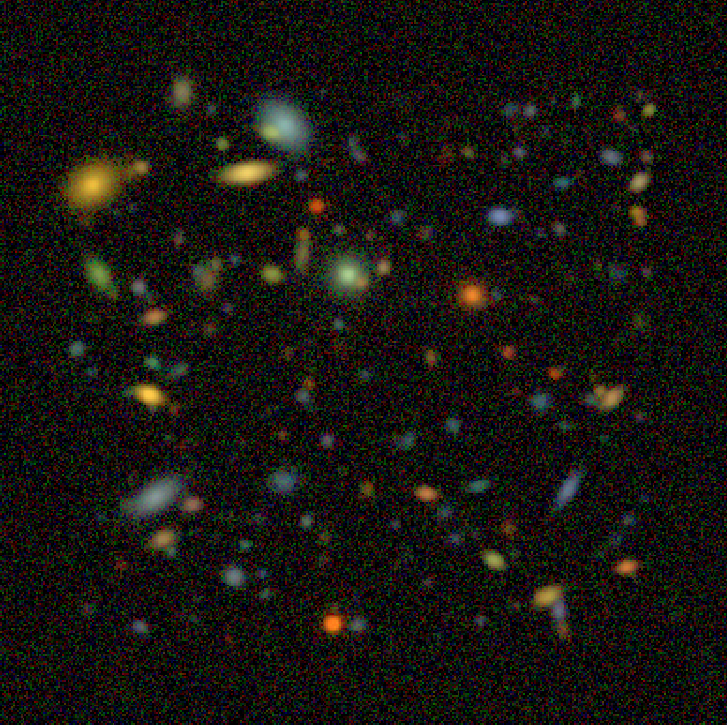
\includegraphics[width=0.9\columnwidth]{figures/lsst-rgb-000003-crop.png}

    \caption{Example images from the DES (left) and LSST (right) simulations.  \label{fig:simimages} }

\end{figure*}



\section{Shear-dependent Detection Biases}

\subsection{Bias in Simulations of Galaxy Pairs}

We tested \mcal\ with MOF deblending using the galaxy pair simulation presented
in \S \ref{sec:pairs}.  Detection was performed using \sx, with settings
matching those used for DES year 5 survey reductions \ess{ref}.  We got similar
results using a simple local peak finder for detection.

The multiplicative bias $m$ is shown in figure \ref{fig:pairbias} as a function
of the pair distance.  For a large separation of 4 arcsec, two objects are
detected in essentially all cases and no significant bias is seen.  For smaller
separations, the two objects overlap more significantly and the detection
becomes more ambiguous, with only one object detected in some cases.  The bias
grows as the separation decreases, with the maximum bias occurring at about 1.5
arcsec separation.  At 1.5 arcsec separation the detection is most ambiguous,
with two objects detected in half the cases.  For smaller separations the
objects overlap more and detection becomes less ambiguous, with one object
detected in more than half of the cases.  At separations of 1 arcsec, the two
objects are detected as one essentially in every case, and again no significant
bias is detected.

\begin{figure}
    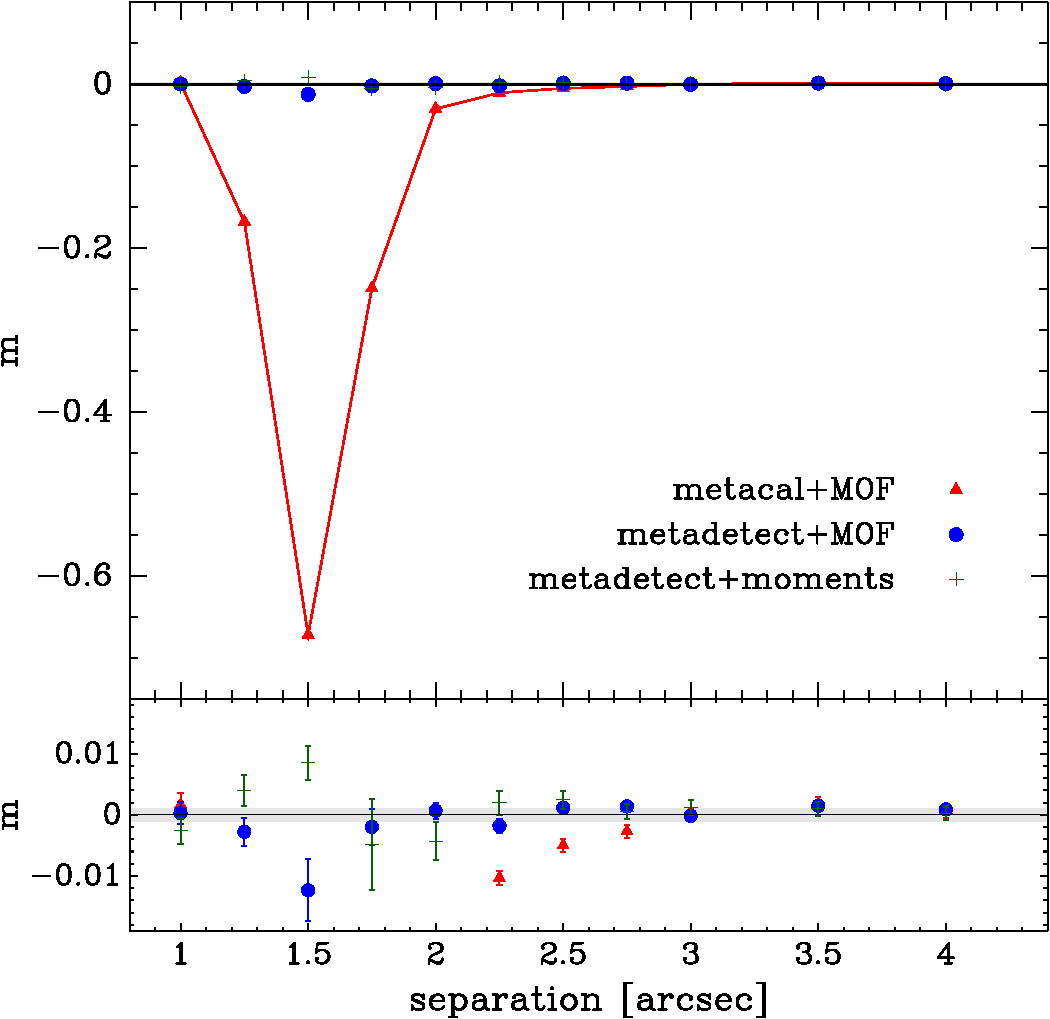
\includegraphics[width=\columnwidth]{figures/pairs-mc-bdkpair.pdf}

    \caption{ Mean multiplicative shear bias measured for pairs of simulated
    galaxies (see \S \ref {sec:pairs} for details) at various separations.  At
    each separation, a large number of trials was generated with random
    orientations of the pair.  At 4.0 arcsec separation, two objects were
    detected in all cases.  At 1.5 arcseconds two objects were detected in half
    the cases.  At 1.0 arcsec a single object was detected in all cases.  Red
    triangles represent standard \mcal\ with MOF deblending for modeling all
    detected objects.  Blue circles represent \mcal+MOF with detection included
    as part of the process.  Green pluses represent \mcal\ with detection
    included but without deblending, and using simple weighted moments without
    PSF correction as the shear estimator. Very large biases are seen for
    standard \mcal+MOF as detection becomes ambiguous, for example at 1.5
    arcsec separations.  When detection is included in the \mcal\ process the
    biases are greatly reduced.  The bias is reduced even in the case where no
    deblending was performed and no PSF correction or detailed object modeling
    were performed.  This indicates the bias is due to shear-dependent
    detection, not light blending or details of the object modeling.
    \label{fig:pairbias}}

\end{figure}

The correspondence between detection ambiguity and shear bias is a hint that
the bias is caused by shear-dependent detection.  As we will show in \S
\ref{sec:mdetpairs}, we can correct this bias by including detection in the
\mcal\ process, even if no explicit deblending is performed.

\subsection{Bias in Simulations with Representative Galaxy Density and Noise}

Erin's tests with WeakLensingDeblending and Matt's tests

\begin{table}
    \centering
    \begin{tabular}{|l|l|c|c|}
        \hline
        Sim & Method         & \snr\ Cut & m             \\
        \hline
        \hline
        DES & MOF+metacal    & \snr$ > 10$ & $-0.016 \pm 0.003$  \\
        DES & MOF+metacal    & \snr$ > 15$ & $-0.038 \pm 0.003$  \\
        DES & MOF+metacal    & \snr$ > 20$ & $-0.053 \pm 0.003$  \\
        \hline
        LSST  & MOF+metacal    & \snr$ > 10$ & $-0.131 \pm 0.005$  \\
        LSST  & MOF+metacal    & \snr$ > 15$ & $-0.124 \pm 0.005$  \\
        LSST  & MOF+metacal    & \snr$ > 20$ & $-0.149 \pm 0.005$  \\
        \hline


    \end{tabular}

    \caption{
            Bias for standard \mcal\ with MOF deblending in simulations with
            realistic galaxy size, flux and noise.  In all cases a cut of
            $T/T_{PSF} > 0.5$ was also applied.  \esstodo{numbers are placeholders,
            need to run regular MOF+metacal on descwl sims}
            \label{tab:mcal:deblending}
    }

\end{table}


\section{Mitigating Shear-dependent Detection Biases with \textsc{METACALIBRATION}}
blah

\subsection{Results for Simulated Galaxy Pairs} \label{sec:mdetpairs}

In figure \ref{fig:pairbias} we show results for pairs of galaxies, including
detection in the \mcal\ process.   The blue filled circles represent the case
where deblending is performed using MOF.  The green plus signs represent the
case where no deblending was performed. For the undeblended case we further
simplified the process:  simple weighted moments were taken at the position
determined by \sx\ using a fixed weight function with full-width at half maximum
1.2 arcsec, without any correction for the PSF.

In both cases the bias is greatly reduced, with significant bias seen only at
the special separation of 1.5 arcsec, where the two objects are detected as one
object in half of the cases.  This demonstrates that the bias we see is not
primarily due to the process of deblending itself, but rather shear-dependent
detection effects.  The remaining biases at 1.5 arcsec tend to be different
sign for the deblended and non-deblended cases, which shows there is a
qualitative difference in how the two measurements respond to the shear. As we
will show below, we find no significant bias for more realistic DES and
LSST-like images where the typical separation of galaxies is not at a special
location of maximum detection ambiguity.

\subsection{Results for Simulations with Representative Galaxy Density and Noise}
\label{sec:res:constpsf}

Erin's results with WeakLensingDeblending and Matt's tests without
psf variation or masking

\begin{table}
    \centering
    \begin{tabular}{|l|l|c|c|}
        \hline
        Sim & Method         & \snr\ Cut & m             \\
        \hline
        \hline
        DES & \mdet+moments & \snr$ > 10$ & $-0.0010 \pm 0.0013$  \\
        DES & \mdet+moments & \snr$ > 15$ & $+0.0000 \pm 0.0013$  \\
        DES & \mdet+moments & \snr$ > 20$ & $+0.0002 \pm 0.0013$  \\
        \hline
        LSST  & \mdet+moments & \snr$ > 10$ & $-0.0027 \pm 0.0011$  \\
        LSST  & \mdet+moments & \snr$ > 15$ & $-0.0018 \pm 0.0011$  \\
        LSST  & \mdet+moments & \snr$ > 20$ & $+0.0001 \pm 0.0011$  \\
        \hline


    \end{tabular}

    \caption{
        Bias for \mcal, including detection in the process (a.k.a. \mdet).  These
        simulations have no PSF variation or masking.  No
        deblending was performed, and simple weighted moments were used
        without PSF correction.  In all cases a cut of $T/T_{PSF} > 0.5$ was
        also applied.  \esstodo{LSST needs to be redone with better
        psf handling.  } \label{tab:mdet:constpsf}
    }

\end{table}



\subsection{Results for Simulations with Realistic Masking and PSF Variation}
\label{sec:res:varpsf}

Matt's stuff with the full glory.  If all are equally unbiased, we can remove
section \ref{sec:res:constpsf}

\mrb{Do we want to show masking?}

\begin{table}
    \centering
    \begin{tabular}{|l|l|c|c|}
        \hline
        Sim & Method         & \snr\ Cut & m             \\
        \hline
        \hline
        DES & \mdet+moments & \snr$ > 10$ & $-0.0010 \pm 0.0013$  \\
        DES & \mdet+moments & \snr$ > 15$ & $+0.0000 \pm 0.0013$  \\
        DES & \mdet+moments & \snr$ > 20$ & $+0.0002 \pm 0.0013$  \\
        \hline
        LSST  & \mdet+moments & \snr$ > 10$ & $-0.0027 \pm 0.0011$  \\
        LSST  & \mdet+moments & \snr$ > 15$ & $-0.0018 \pm 0.0011$  \\
        LSST  & \mdet+moments & \snr$ > 20$ & $+0.0001 \pm 0.0011$  \\
        \hline


    \end{tabular}

    \caption{
        Same as table \ref{tab:mdet:constpsf} but with realistic masking and
        spatial PSF variation.  \esstodo{numbers are placeholders} \label{tab:mdet:varpsf}
    }

\end{table}


\section{Summary}
blah

\bibliographystyle{mnras}
\bibliography{references}

\appendix

\section{Fast Approximate Variable PSF Models}

In this work we use a fast, approximate variable PSF model. This model eases the
computational requirements for the simulations while also retaining the
essential features of realistic PSF variation. In this appendix, we present
the model and verify its statistical properties against more realistic PSF models.

We start with the results of \citet{heymans2012}. They fit the \vonkarman model
of atmospheric turbulence

\begin{displaymath}
  P(\ell) \propto \left(\ell^{2} + \frac{1}{\theta_{0}^2}\right)^{-11/6}
\end{displaymath}
to images with high stellar density. Here $\theta_{0}$ is the outer scale of
turbulence. \citep{heymans2012} find that $\theta_{0}\approx3$ arcmin.
We further add an additional Gaussian truncation of the power

\begin{displaymath}
  P_{trunc}(\ell) \propto P(\ell)\exp\left(-\ell^2r^{2}\right)
\end{displaymath}
at a scale of $r=1$ arcsec in order to reduce the level of resulting
PSF variation.
\esstodo{How do we justify that?   Based on exposure time?}

Using this model, we seed equal amounts of E- and B-mode power on a grid of
$128\times128$ cells using random phases. Each cell of the grid is one
arcsec in size. We normalize the overall shape variance to $0.05^2$. We then use
the $g1$ and $g2$ components of this model to set the shape of the PSF at each
location. Note that we also bound the total ellipticity to at most 0.5.
We model the PSF profile as a Moffat with shape parameter $\beta=2.5$.
The size of the Moffat profile is set to be proportional to $\mu^{-3/4}$,
where $\mu$ is the magnification computed from the power spectra realization. The
proportionality constant is drawn randomly from a log-normal model with
scatter 0.1 arcmin and a central value set so the final PSF size. This mimics
the typical seeing conditions of a given survey.

We show an example PSF for a DES-like survey in Figure~\ref{fig:pspsf}.  Over a
1 square arcminute patch, our approximate models generate PSF shape and size
variation that are $\gtrsim10\times$ that seen in real 90 second exposures
with DECam \mrb{ref}, or the expected variation in a 15 second exposure with
LSST \mrb{ref}.  Figure~\ref{fig:psxi} shows the $\xi_{\pm}$ shear correlation
functions averaged over 100 realizations of our models. For comparison, we
expect at most shear correlation function amplitudes of $\sim10^{-4}$ for LSST
\mrb{ref} and for DESCam 90 second exposures. The DECam models were generated
using the methods of \mrb{ref} but for DECam-like environmental conditions. For
the optical contributions to the PSF, we use a set of randomly drawn
aberrations (similar to GREAT3 \mrb{ref}), but with values more typical of
DECam
observations\footnote{\url{https://github.com/GalSim-developers/GalSim/blob/releases/2.1/examples/great3/cgc.yaml}}.
Finally, we note that simulations of metadetection with this PSF model show
$\approx-0.8\%$ multiplicative biases.
\esstodo{What 0.8\% for LSST depth?  Are you using smaller variations for
the LSST sims to show we are ok for LSST?}

\begin{figure*}
  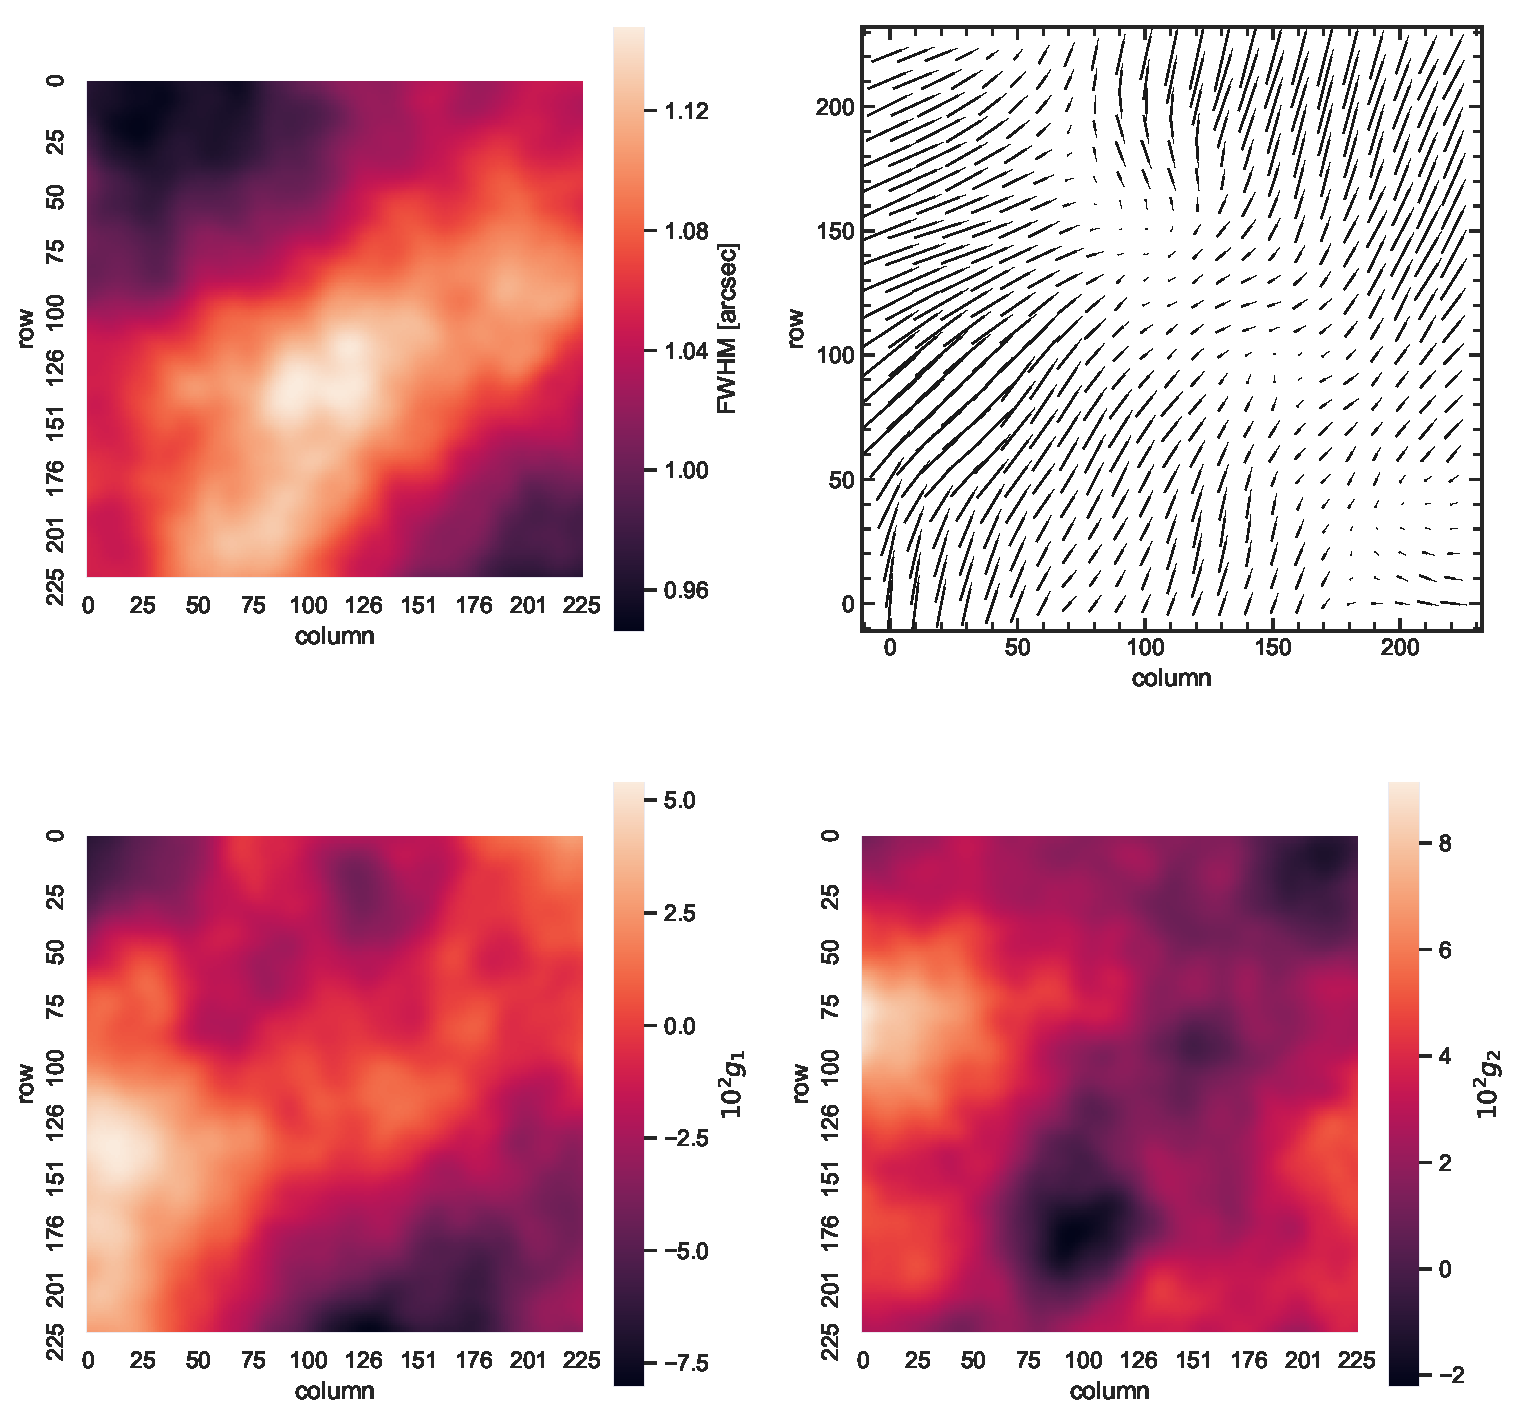
\includegraphics[width=\textwidth]{figures/pspsf.pdf}
  \caption{
    Variable PSF model statistics for a DECam-like exposure. The top-left
    panel shows the variation in the FWHM in arcseconds. The top-right panel
    shows a visualization of the PSF shape variation. The bottom-left panel shows
    the variation in the $1$-component of the PSF shape. The bottom-right panel
    shows the variation in the $2$-component of the PSF shape. The variation in
    this model is $\gtrsim10\times$ larger than the typical PSF variation for
    either DECam or expected LSST observations.
    \label{fig:pspsf}}
\end{figure*}

\begin{figure}
  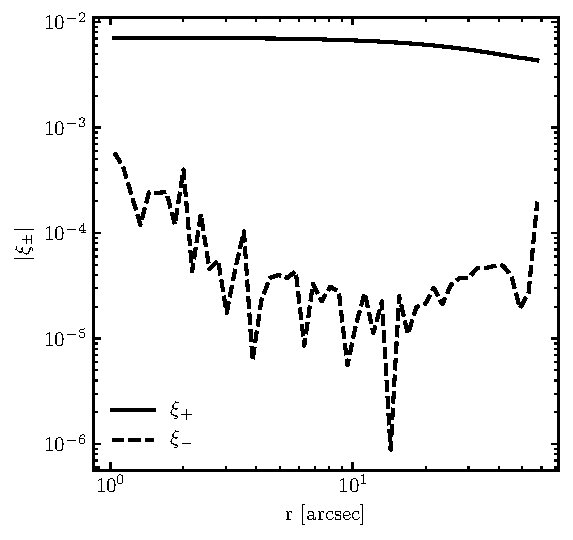
\includegraphics[width=\columnwidth]{figures/psxi.pdf}
  \caption{
    Variable PSF model shear correlation functions for a DECam-like exposure. LSST
    is expected to have shear correlation function magnitudes around
    $\sim10^{-4}$ \mrb{ref}.
    \label{fig:psxi}}
\end{figure}


\bsp
\label{lastpage}
\end{document}
